\begin{center}
\scriptsize
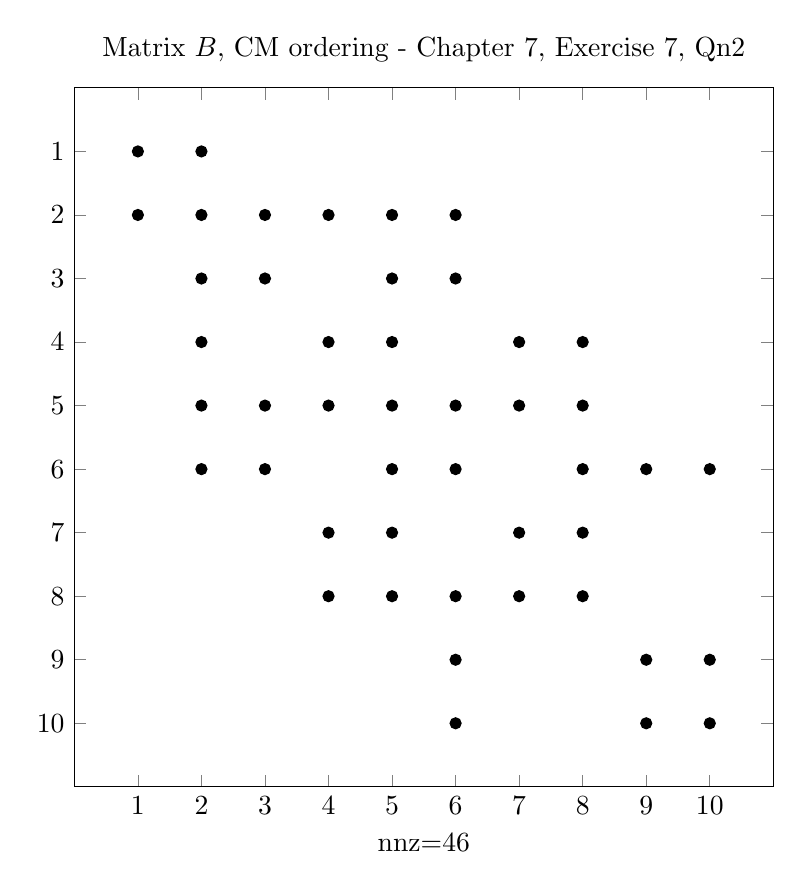
\begin{tikzpicture}
    [   baseline = {(current bounding box.north)}
    ]
    \begin{axis}
        [   unit vector ratio* = 1 1 1
        ,   y dir = reverse
        ,   xmin = 0
        ,   ymin = 0
        ,   xmax = 11
        ,   ymax = 11
        ,   title = {Matrix $B$, CM ordering - Chapter 7, Exercise 7, Qn2}
        ,   xlabel = {nnz=46}
        ,   width = \linewidth
        ,   xtick = {1,2,3,4,5,6,7,8,9,10}
        ,   ytick = {1,2,3,4,5,6,7,8,9,10}
        ]
        \addplot[only marks] coordinates
        {   (1,1)(2,1)
            (1,2)(2,2)(3,2)(4,2)(5,2)(6,2)
                 (2,3)(3,3)     (5,3)(6,3)
                 (2,4)     (4,4)(5,4)     (7,4)(8,4)
                 (2,5)(3,5)(4,5)(5,5)(6,5)(7,5)(8,5)
                 (2,6)(3,6)     (5,6)(6,6)     (8,6)(9,6)(10,6)
                           (4,7)(5,7)     (7,7)(8,7)
                           (4,8)(5,8)(6,8)(7,8)(8,8)
                                     (6,9)          (9,9)(10,9)
                                     (6,10)        (9,10)(10,10)
        };
    \end{axis}
\end{tikzpicture}
\end{center}
